% Copyright (C) 2008-2010 Rosita Wachenchauzer <rositaw@gmail.com>
%               Maximiliano Curia <maxy@gnuservers.com.ar>
%               Margarita Manterola <margamanterola@gmail.com>

% Esta obra está licenciada de forma dual, bajo las licencias Creative
% Commons:
%  * Atribución-Compartir Obras Derivadas Igual 2.5 Argentina
%    http://creativecommons.org/licenses/by-sa/2.5/ar/
%  * Atribución-Compartir Obras Derivadas Igual 3.0 Unported
%    http://creativecommons.org/licenses/by-sa/3.0/deed.es_AR.
%
% A su criterio, puede utilizar una u otra licencia, o las dos.
% Para ver una copia de las licencias, puede visitar los sitios
% mencionados, o enviar una carta a Creative Commons,
% 171 Second Street, Suite 300, San Francisco, California, 94105, USA.

\chapter{Polimorfismo, Herencia y Delegación}

En esta unidad veremos algunos temas que son centrales a la programación
orientada a objetos: polimorfismo, herencia y delegación.

\section{Polimorfismo}

El concepto de {\it polimorfismo} (del griego {\it muchas formas}) implica
que si en una porción de código se invoca un determinado método de un
objeto, podrán obtenerse distintos resultados según la clase del objeto.
Esto se debe a que distintos objetos pueden tener un método con un mismo
nombre, pero que realice distintas operaciones.

En las unidades anteriores, varias veces utilizamos las posibilidades
provistas por el polimorfismo, sin haberle puesto este nombre.

Se vio, por ejemplo, que es posible recorrer cualquier tipo de secuencia
(ya sea una lista, una tupla, un diccionario, un archivo o cualquier otro tipo
de secuencia) utilizando la misma estructura de código
(\lstinline!for elemento in secuencia!).

De la misma forma, hemos utilizado funciones que podían trabajar con los
distintos tipos numéricos sin hacer distinción sobre de qué tipo de número
se trataba (entero, real, largo o complejo).

Por otro lado, en la unidad anterior se vio también que al construir una
clase, es posible incluir el método \lstinline!__str__! para que cuando se
quiera imprimir el objeto se lo haga de la forma deseada; así como una
gran variedad de otros métodos especiales, que permiten que operadores
comunes sean utilizados sobre distintos tipos de objetos.

\subsection{Interfaz}

Llamamos {\bf interfaz} a un conjunto de funciones, métodos o atributos con
nombres específicos.  Una interfaz es un {\it contrato} entre el
programador que realiza una clase y el que la utiliza, puede consistir en
uno solo o varios métodos o atributos.

Por ejemplo, para que un objeto se pueda comparar con otros, debe cumplir
con la interfaz {\it comparable}, que en Python implica incluir el método
\lstinline!__cmp__! visto en la unidad anterior.

La idea de polimorfismo se basa, entonces, en utilizar distintos tipos de
datos a través de una interfaz común.

\subsection{Redefinición de métodos}

Llamamos {\bf redefinición} a la acción de definir un método con el mismo
nombre en distintas clases, de forma tal que provea una interfaz.

Un bloque de código será {\it polimórfico} cuando dentro de ese código se
realicen llamadas a métodos que puedan estar redefinidos en distintas
clases.

Tomemos por ejemplo el caso ya mencionado en el que se recorre una
secuencia (lista, tupla, archivo, etc) mediante una misma estructura de
código.  Esto es posible gracias a la redefinición del método especial
\lstinline!__iter__!, que devuelve un {\it iterador}.  Un bloque que
utiliza una secuencia en forma genérica es, entonces, un bloque
polimórfico.

\begin{sabias_que}
En Python al no ser necesario especificar explícitamente el tipo de los
parámetros que recibe una función, las funciones son naturalmente
polimórficas.

En otros lenguajes, puede darse que sólo algunas funciones específicas sean
polimórficas (como en C++, por ejemplo), o que sea extremadamente difícil
obtener un comportamiento polimórfico (como es el caso de C).
\end{sabias_que}

En la vida real, cuando analizamos las funciones de respiración,
reproducción o alimentación, de los seres vivos vemos que siempre se repite
el mismo patrón: si bien la acción en todos los casos es la misma, puede
suceder que haya diferencias en la {\it implementación} en cada tipo, ya
que no es lo mismo la respiración de una mojarrita que la de un malvón, no
es lo mismo la reproducción de una ameba que la de un elefante.

De la misma forma, al implementar nuestras clases, debemos proveer
distintas implementaciones de los métodos que se llaman igual, para que
puedan comportarse polimórficamente, como ser las redefiniciones de los
métodos \lstinline!__str__! o \lstinline!__cmp__! vistas en la unidad
anterior.

En particular en Python, la {\it sobrecarga de operadores}, mencionada
anteriormente,  es un proceso que se realiza mediante la redefinición de
algunos métodos especiales.  En otros lenguajes se utilizan técnicas distintas
para obtener el mismo resultado.

\begin{sabias_que}
El término {\it sobrecarga} viene de un posible uso de polimorfismo que
está presente en algunos lenguajes orientados a objetos: la posibilidad de
tener, dentro de una misma clase, dos métodos que se llamen igual pero
reciban parámetros de distintos tipos.  Es decir, que el método al que hay
que llamar se decide por el tipo del parámetro, no por el tipo del objeto
que lo contiene.

En Python no tenemos sobrecarga de métodos, ya que al no definir los tipos
de los parámetros en el encabezado, no sería posible distinguir a qué
método hay que llamar.  Sin embargo, se puede decir que sí tenemos
sobrecarga de operadores, ya que al encontrar un operador, Python llamará a
distintos métodos según el tipo de las variables que se quiera sumar,
restar, multiplicar, etc.
\end{sabias_que}

\subsection{Un ejemplo de polimorfismo}

En la unidad anterior se vio la clase \lstinline!Punto! que representa a un
punto en el plano.  Es posible definir también una clase
\lstinline!Punto3D!, que represente un punto en el espacio.  Esta nueva
clase contendrá los mismos métodos que se vieron para \lstinline!Punto!,
pero para tres coordenadas.

Si a ambas clases le agregamos un método para multiplicar por un escalar
(\lstinline!__mul__(self, escalar)!), podríamos tener la siguiente función
polimórfica:

\begin{codigo-python-sn}
def obtener_versor(punto):
    norma = punto.norma()
    return punto * (1.0 / norma)
\end{codigo-python-sn}

Esta función devolverá un versor de dos dimensiones o de tres dimensiones,
según a qué clase pertenezca la variable \lstinline!punto!.

\begin{atencion}
A veces puede suceder que una función polimórfica imponga alguna
restricción sobre los tipos de los parámetros sobre los que opera. En el
ejemplo anterior, el objeto \lstinline!punto! debe tener el método
\lstinline!norma! y la posibilidad de multiplicarlo por un escalar.
\end{atencion}

Otro ejemplo que ya hemos visto, utilizando secuencias, es usar un
diccionario para contar la frecuencia de aparación de elementos dentro de
una secuencia cualquiera.

\begin{codigo-python}
def frecuencias(secuencia):
    """ Calcula las frecuencias de aparición de los elementos de
        la secuencia recibida.
        Devuelve un diccionario con elementos: {valor: frecuencia}
    """
    # crea un diccionario vacío
    frec = dict()
    # recorre la secuencia
    for elemento in secuencia:
        frec[elemento] = frec.get(elemento, 0) + 1
    return frec
\end{codigo-python}

Vemos que el parámetro \lstinline!secuencia! puede ser de cualquier tipo
que se encuentre dentro de la ``familia'' de las secuencias. En cambio, si
llamamos a la función con un entero se levanta una excepción.

\begin{codigo-python-sn}
>>> frecuencias(["peras", "manzanas", "peras", "manzanas", "uvas"])
{'uvas': 1, 'peras': 2, 'manzanas': 2}
>>> frecuencias((1,3,4,2,3,1))
{1: 2, 2: 1, 3: 2, 4: 1}
>>> frecuencias("Una frase")
{'a': 2, ' ': 1, 'e': 1, 'f': 1, 'n': 1, 's': 1, 'r': 1, 'U': 1}
>>> ran = xrange(3, 10, 2)
>>> frecuencias(ran)
{9: 1, 3: 1, 5: 1, 7: 1}
>>> frecuencias(4)
Traceback (most recent call last):
  File "<pyshell#0>", line 1, in <module>
    frecuencias(4)
  File "frecuencias.py", line 12, in frecuencias
    for v in seq:
TypeError: 'int' object is not iterable
\end{codigo-python-sn}

\section{Herencia}

La {\it herencia} es un mecanismo de la programación orientada a objetos que
sirve para crear clases nuevas a partir de clases preexistentes.  Se toman
({\it heredan}) atributos y comportamientos de las clases viejas y se los
modifica para modelar una nueva situación.

La clase vieja se llama {\it clase base} y la que se construye a partir de
ella es una {\it clase derivada}.

Por ejemplo, a partir de una clase \lstinline!Persona! (que contenga como
atributos \lstinline!identificacion!, \lstinline!nombre!, \lstinline!apellido!)
podemos construir la clase \lstinline!AlumnoFIUBA! que extiende a
\lstinline!Persona! y agrega como atributo el \lstinline!padron!.

Para indicar el nombre de la clase base, se la pone entre paréntesis a
continuación del nombre de la clase (en lugar de la expresión
\lstinline!object! que poníamos anteriormente --en realidad \lstinline!object!
es el nombre de la clase base genérica--).

Definimos \lstinline!Persona!:
\begin{codigo-python-sn}
class Persona(object):
    "Clase que representa una persona."
    def __init__(self, identificacion, nombre, apellido):
        "Constructor de Persona"
        self.identificacion = identificacion
        self.nombre = nombre
        self.apellido = apellido
    def __str__(self):
        return "%s: %s, %s" % \
            (str(self.identificacion), self.apellido, self.nombre)
\end{codigo-python-sn}

A continuación definimos \lstinline!AlumnoFIUBA! como derivada de
\lstinline!Persona!, de forma tal que inicialice el nuevo atributo, pero a su
vez utilice la inicialización de \lstinline!Persona! para las atributos de la
clase base:

\begin{codigo-python-sn}
class AlumnoFIUBA(Persona):
    "Clase que representa a un alumno de FIUBA."
    def __init__(self, identificacion, nombre, apellido, padron):
        "Constructor de AlumnoFIUBA"
        # llamamos al constructor de Persona
        Persona.__init__(self, identificacion, nombre, apellido)
        # agregamos el nuevo atributo
        self.padron = padron
\end{codigo-python-sn}

Probamos la nueva clase:

\begin{codigo-python-sn}
>>> a = AlumnoFIUBA("DNI 35123456", "Damien", "Thorn", "98765")
>>> print a
DNI 35123456: Thorn, Damien
\end{codigo-python-sn}

Vemos que se heredó el método \lstinline+__str__+ de la clase base. Si
queremos, podemos redefinirlo:

\begin{codigo-python-sn}
    def __str__(self):
        "Devuelve una cadena representativa del alumno"
        return "%d: %s, %s" % \
            (str(self.padron), self.apellido, self.nombre)
\end{codigo-python-sn}

Volvemos a probar:

\begin{codigo-python-sn}
>>> a = AlumnoFIUBA("DNI 35123456", "Damien", "Thorn", "98765")
>>> print a
98765: Thorn, Damien
\end{codigo-python-sn}

De una clase base se pueden construir muchas clases derivadas, así como
hemos derivado alumnos, podríamos derivar docentes, empleados, clientes,
proveedores, o lo que fuera necesario según la aplicación que estemos
desarrollando.

\begin{sabias_que}
En el diseño de jerarquias de herencia no siempre es del todo fácil decidir
cuándo una clase debe extender a otra.
La regla práctica para decidir si una clase (S) puede ser
definida como heredera de otra (T) es que debe cumplirse que ``S es un T''.
Por ejemplo, {\it Perro} es un {\it Animal}, pero {\it Vehículo} no es un {\it
Motor}.

Esta regla se desprende del principio de sustitución de Liskov (formulado por
Barbara Liskov y Jeannette Wing).

Barbara Liskov es una mujer importante en la historia de la informática, no
sólo por este principio, sino que fue la primera mujer en recibir un doctorado
en las ciencias de la computación, creadora de varios lenguajes y actualmente
es profesora e investigadora del MIT.
\end{sabias_que}

En el caso de Python, también se puede construir una clase derivada a partir de
varias clases base (por ejemplo, un ayudante de segunda en la UBA es un alumno
que también trabaja de docente).  Esta posbilidad se llama {\bf Herencia
Múltiple}, pero no la detallaremos por ahora.

\subsection*{La clase de las figuras}

Un ejemplo clásico de herencia es el de las figuras cerradas en el plano, con un
método para calcular el área. En este caso, la clase base no tiene comportamiento definido
ni atributos, dado que cada figura tiene atributos muy distintos (radio en el caso
del círculo, base y altura en el caso del triángulo, etc.), y en cuanto al cálculo
del área, cada figura tiene una fórmula diferente:

\begin{itemize}
\item La clase base:

\begin{codigo-python-sn}
class Figura(object):
    """ Una figura en el plano. """
    def area(self):
        " Este método debe ser redefinido. "
        pass
\end{codigo-python-sn}

\item Los círculos:

\begin{codigo-python-sn}
from math import pi

class Circulo(Figura):
    """ Un círculo en el plano. """
    def __init__(self, radio=0):
        " Constructor de círculo. "
        self.radio = radio

    def area(self):
        " Devuelve el área del círculo. "
        return pi * self.radio * self.radio
\end{codigo-python-sn}

\item Y los triángulos:

\begin{codigo-python-sn}
class Triangulo(Figura):
    """ Un triángulo en el plano. """
    def __init__(self, base=0, altura=0):
        " Constructor de triángulo. "
        self.base = base
        self.altura = altura

    def area(self):
        " Devuelve el área del triángulo. "
        return self.base * self.altura / 2.
\end{codigo-python-sn}

\end{itemize}

Y ahora las pruebas:
\begin{codigo-python-sn}
>>> c = Circulo(4)
>>> c.area()
50.26548245743669
>>>
>>> t = Triangulo(3, 5)
>>> t.area()
7.5
\end{codigo-python-sn}

\section{Delegación}

Llamamos delegación a la situación en la que una clase contiene (como
atributos) una o más instancias de otra clase, a las que {\it delegará}
parte de sus funcionalidades. Esta relación entre clases suele ser la más
indicada cuando es necesaria una asociación entre las clases pero el
principio de Liskov no se cumple. También puede verse como la relación
entre clases ``S contiene a T''. Por ejemplo, Vehículo {\bf contiene} un
Motor, pero Alumno no contiene a Persona, sino que {\bf es} una Persona. \\

Por ejemplo, la clase \lstinline!Hotel! vista en la unidad anterior, podría
contener una clase \lstinline!Disponibilidad!, que almacene la
disponibilidad de las habitaciones del hotel para distintas fechas.  La
clase \lstinline!Hotel! debería tener, entonces, los métodos
\lstinline!consultar_disponibilidad!, \lstinline!reservar! y
\lstinline!cancelar!, que todos delegarían en la clase
\lstinline!Disponibilidad! su funcionamiento principal.

% TODO: completar el ejemplo.

%\ejercicioc{Programar una clase \verb+DisponibilidadHotel+ contenida en \verb+Hotel+
%que tenga un calendario de disponibilidades de un hotel y donde se puedan hacer
%reservas para una fecha dada.}

%\ejercicioc{Se necesita una clase que permita ver la disponibilidad hotelera
%de una ciudad,
%y que cuente con un método {\tt aconsejar} que, para una
%fecha dada, aconseje cuáles son los hoteles disponibles ordenados de mayor
%a menor por la relación calidad--precio. Debe permitir reservar una habitación
%en el hotel elegido.}

\subsection*{Delegación y Referencias}

Queremos construir una clase \lstinline!Rectangulo!, que se describe
mediante los siguientes atributos:

\begin{itemize}
\item {\bf Longitud de su base}: un número.

\item {\bf Longitud de su altura}: un número.

\item {\bf El punto del plano de su esquina inferior izquierda}: un punto del plano.

\end{itemize}

Incluiremos métodos para inicializar y mostrar, para calcular el área y
para trasladar el rectángulo en el plano.

\begin{codigo}{Rectangulo.py}{Clase para modelar un Rectángulo}
\label{Rectangulo}
\lstinputlisting{src/15_herencia_polimorf/Rectangulo.py}
\end{codigo}

La implementación básica puede verse en el Código \ref{Rectangulo}.  Se
puede ver que el rectángulo realiza internamente la operación para calcular
el área, pero para la operación del traslado, delega la suma de los puntos
al operador \lstinline!__add__! de la clase \lstinline!Punto!.

Recordamos que cuando se hace \lstinline!self.origen + Punto(dx,dy)!,
Python llama al método \lstinline!__add__! de la clase \lstinline!Punto!,
que recibe los dos puntos y devuelve un nuevo punto con la suma de ambos.

Para construir y utilizar el rectángulo, lo haremos de la siguiente forma:

\begin{codigo-python-sn}
>>> from Punto import Punto
>>> from Rectangulo import Rectangulo
>>> r = Rectangulo(2, 3, Punto(1, 2))
>>> print r
Base: 2, Altura: 3, Esquina inf. izq.: (1, 2)
>>> print r.area()
6
\end{codigo-python-sn}

Lo que acabamos de crear es un objeto de acuerdo al siguiente diagrama que
se muestra en la Figura \ref{rectangulo_punto}.

\begin{figure}[htb]
\label{rectangulo_punto}
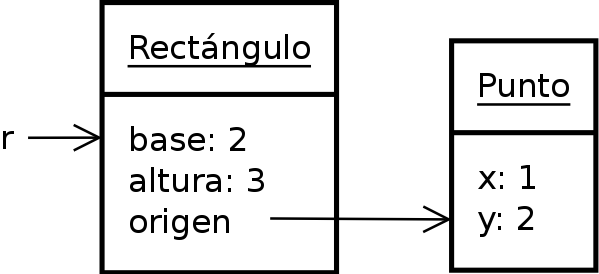
\includegraphics{graficos/15_Rectangulo_Punto}
\caption{Estado de las variables, al momento de crear el rectángulo}
\end{figure}

El punto que describe la posición de la esquina inferior izquierda del
rectángulo es un objeto \lstinline!Punto!. El atributo \lstinline!origen!
contiene una {\it referencia} a dicho objeto.

Utilizando el método \lstinline!trasladar!, podemos modificar el valor del
punto contenido dentro del rectángulo.

\begin{codigo-python-sn}
>>> r.trasladar(2,4)
>>> print r
Base: 2, Altura: 3, Esquina inf. izq.: (3, 6)
\end{codigo-python-sn}

También es posible directamente reemplazar el punto contenido, por un nuevo
punto.

\begin{codigo-python-sn}
>>> q = Punto(7,2)
>>> r.origen = q
>>> print r
Base: 2, Altura: 3, Esquina inf. izq.: (7, 2)
\end{codigo-python-sn}

Con lo cual el diagrama pasa a ser el de la Figura
\ref{rectangulo_punto_b}.

\begin{figure}[htb]
\label{rectangulo_punto_b}
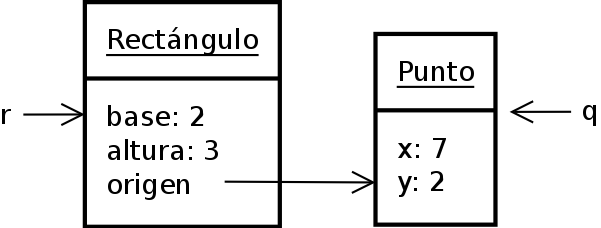
\includegraphics{graficos/15_Rectangulo_Punto_b}
\caption{Estado de las variables, luego de reemplazar el origen}
\end{figure}

\begin{observacion}
El \lstinline!Punto(1, 2)! y \lstinline!Punto(3,6)! que habían sido creados
previamente, están ahora fuera de uso, por lo que quedan a disposición de un
mecanismo de {\it recolección de basura}, que no es tema de esta materia,
que se encarga de juntar todos los pedazos de memoria que se descartan
durante la ejecución de un programa.
\end{observacion}

\section{Resumen}

\begin{itemize}
\item Se llama {\bf polimorfismo} a la posibilidad de obtener distintos
comportamientos mediante la invocación a métodos de un mismo nombre, pero de
clases distintas.

\item Se llama {\bf herencia} a la relación entre clases en la cual una es una
clase base y otra es una clase derivada, que {\it hereda} los métodos y
atributos de la clase base.

\item Se llama {\bf delegación} a la relación entre clases en la cual una clase
contiene como atributo a otra clase, y dentro de sus métodos realiza
invocaciones a los métodos de la clase contenida.

\item Se denomina {\bf referencia} a las variables que permiten acceder a
un determinado objeto, ya sea un atributo dentro de un objeto, o una
variable en una porción de código cualquiera.
\end{itemize}


\newpage
\section{Ejercicios}

\extractionlabel{guia}
\begin{ejercicio}
{\bf Papel, Birome, Marcador}
\begin{partes}
    \item Escribir una clase {\it Papel} que contenga un texto, un método {\it
escribir}, que reciba una cadena para agregar al texto, y el método {\it
\_\_str\_\_} que imprima el contenido del texto.
    \item Escribir una clase {\it Birome} que contenga una cantidad de tinta, y
un método {\it escribir}, que reciba un texto y un papel sobre el cual
escribir. Cada letra escrita debe reducir la cantidad de tinta contenida.
Cuando la tinta se acabe, debe lanzar una excepción.
    \item Escribir una clase {\it Marcador} que herede de Birome, y agregue el
método {\it recargar}, que reciba la cantidad de tinta a agregar.
\end{partes}
\end{ejercicio}


\extractionlabel{guia}
\begin{ejercicio}
{\bf Juego de Rol}
\begin{partes}
    \item Escribir una clase {\it Personaje} que contenga los atributos {\it
vida}, {\it posicion} y {\it velocidad}, y los métodos {\it
recibir\_ataque}, que reduzca la vida según una cantidad recibida y lance
una excepción si la vida pasa a ser menor o igual que cero, y {\it
mover} que reciba una dirección y se mueva en esa dirección la cantidad
indicada por velocidad.
    \item Escribir una clase {\it Soldado} que herede de Personaje, y agregue
el atributo {\it ataque} y el método {\it atacar}, que reciba otro
personaje, al que le debe hacer el daño indicado por el atributo ataque.
    \item Escribir una clase {\it Campesino} que herede de Personaje, y agregue
el atributo {\it cosecha} y el método {\it cosechar}, que devuelva la
cantidad cosechada.
\end{partes}
\end{ejercicio}

